\section{Kernel methods}

Frequently, we seek to detect nonlinear patterns within our datasets. 
In nonlinear regression, the connection between input and output may deviate from linearity, while in nonlinear classification, class boundaries might not be linearly separable. 
Linear models often prove insufficient in capturing such complexities. 
However, kernel methods offer a solution by transforming data into higher-dimensional spaces where linear relationships become apparent, thereby enabling linear models to effectively operate in nonlinear scenarios.

The process of transforming the original input space into a feature space is termed feature mapping, denoted as:
\[\Phi:x\rightarrow\phi(x)\]

\begin{example}
    Consider a binary classification problem where no linear separator exists:
    \begin{figure}[H]
        \centering
        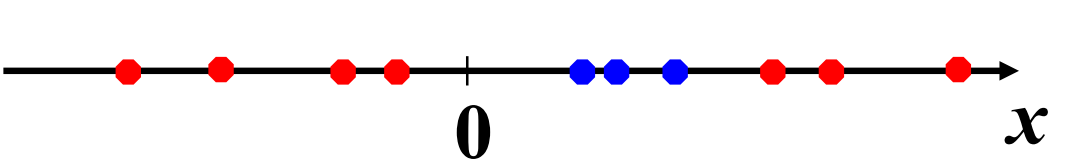
\includegraphics[width=0.5\linewidth]{images/ker1.png}
    \end{figure}
    Now, let's map the input space (a single variable $x$) to a feature space with two features: $x\rightarrow\left\{ x,x^2 \right\}$
    As a result, the data becomes linearly separable:
    \begin{figure}[H]
        \centering
        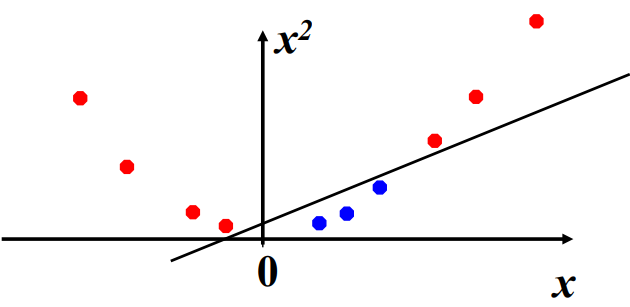
\includegraphics[width=0.5\linewidth]{images/ker2.png}
    \end{figure}
\end{example}
This concept extends naturally to higher dimensions and more intricate problem domains.

However, a significant drawback arises known as the curse of dimensionality. 
This occurs due to the exponential growth in the number of features as the input variables increase, rendering the mapping computationally infeasible.
Kernel methods offer a solution to this challenge by bypassing the need for explicit computation of the feature mapping.
While they are computationally intensive, they remain feasible for practical implementation.

\subsection{Kernel function}
The kernel function is defined as the scalar product between the feature vectors of two data samples:
\[k(\textbf{x},\textbf{x}^\prime)=\phi{(\textbf{x})}^T\phi(\textbf{x})\]
The kernel function exhibits symmetry: $k(\textbf{x},\textbf{x}^\prime)=k(\textbf{x}^\prime,\textbf{x})$.
It can be interpreted as a measure of similarity between $\textbf{x}$ and $\textbf{x}^\prime$.

Interestingly, very large feature vectors, even infinite ones, can result in a kernel function that is computationally tractable.

Certain special classes of kernel functions exist:
\begin{itemize}
    \item \textit{Stationary kernels}: $k(\textbf{x},\textbf{x}^\prime)=k(\textbf{x}-\textbf{x}^\prime)$.
    \item \textit{Homogeneous kernels} (or radial basis functions): $k(\textbf{x},\textbf{x}^\prime)=k(\left\lVert \textbf{x}-\textbf{x}^\prime\right\rVert )$.
\end{itemize}

\paragraph*{Kernel function design}
We are not obligated to compute the kernel function by first generating the feature space, as we aim to avoid explicitly calculating the feature vectors.
Two primary approaches exist for designing a kernel function:
\begin{itemize}
    \item Create kernel functions directly from scratch.
    \item Design kernel functions by applying a predefined set of rules to existing ones.
\end{itemize}
In both cases, it's crucial to ensure that the resulting kernel functions are valid, meaning they correspond to a scalar product in some feature space.
\begin{theorem}[Mercer]
    Any continuous, symmetric, positive semi-definite kernel function $k(\textbf{x},\textbf{x}^\prime)$ can be expressed as a dot product in a high-dimensional space. 
\end{theorem}
For this theorem, the necessary and sufficient condition for a function $k(\textbf{x},\textbf{x}^\prime)$ to be a valid kernel is that the Gram matrix $\textbf{K}$ is positive semi-definite for all possible choices of $\mathcal{D}=\{x_i\}$.
This condition implies that $\textbf{x}^T\textbf{K}\textbf{x}>0$ for any non-zero real vector $\textbf{x}$, meaning that the double sum $\sum_i\sum_j\textbf{K}_{ij}\textbf{x}_i\textbf{x}_j$ is strictly positive for any real numbers $\textbf{x}_i$ and $\textbf{x}_j$.

Given valid kernels $k_1(\textbf{x},\textbf{x}^\prime)$ and $k_2(\textbf{x},\textbf{x}^\prime)$ the following rules can be applied to design a new valid kernel:
\begin{enumerate}
    \item $k_(\textbf{x},\textbf{x}^\prime)=ck_1(\textbf{x},\textbf{x}^\prime)$, where $c>0$ is a constant. 
    \item $k_(\textbf{x},\textbf{x}^\prime)=f(\textbf{x})k_1(\textbf{x},\textbf{x}^\prime)f(\textbf{x}^\prime)$, where $f(\cdot)$ is any function. 
    \item $k_(\textbf{x},\textbf{x}^\prime)=q\left( k_1(\textbf{x},\textbf{x}^\prime) \right)$, where $q(\cdot)$ is a polynomial with non-negative coefficients. 
    \item $k_(\textbf{x},\textbf{x}^\prime)=e^{k_1(\textbf{x},\textbf{x}^\prime)}$. 
    \item $k_(\textbf{x},\textbf{x}^\prime)=k_1(\textbf{x},\textbf{x}^\prime)+k_2(\textbf{x},\textbf{x}^\prime)$. 
    \item $k_(\textbf{x},\textbf{x}^\prime)=k_1(\textbf{x},\textbf{x}^\prime)k_2(\textbf{x},\textbf{x}^\prime)$. 
    \item $k_(\textbf{x},\textbf{x}^\prime)=k_3(\boldsymbol{\phi}(\textbf{x}),\boldsymbol{\phi}(\textbf{x}^\prime))$, where $\boldsymbol{\phi}(\textbf{x})$ maps $\textbf{x}$ to $\mathbb{R}^M$ and $k_3(\cdot,\cdot)$ is a valid kernel in $\mathbb{R}^M$. 
    \item $k_(\textbf{x},\textbf{x}^\prime)=\textbf{x}^T\textbf{A}\textbf{x}$, where $\textbf{A}$ is a symmetric semidefinite matrix. 
    \item $k_(\textbf{x},\textbf{x}^\prime)=k_a(\textbf{x}_a,\textbf{x}_a^\prime)+k_b(\textbf{x}_b,\textbf{x}_b^\prime)$. 
    \item $k_(\textbf{x},\textbf{x}^\prime)=k_a(\textbf{x}_a,\textbf{x}_a^\prime)k_b(\textbf{x}_b,\textbf{x}_b^\prime)$.
\end{enumerate}

\paragraph*{Kernel trick}
It's feasible to modify the representation of linear models by substituting terms involving $\phi(\textbf{x})$ with alternatives solely based on $k(\textbf{x},\cdot)$.
In essence, the output of a linear model can be computed solely based on the similarities between data samples, as computed with the kernel function.

This methodology, known as the kernel trick, finds application in various learning algorithms including: ridge regression, $K-NN$ regression, perceptron, nonlinear PCA, and support vector machines.

\paragraph*{Gaussian kernel}
The Gaussian kernel is a widely employed kernel function in various machine learning algorithms. 
Its mathematical representation is given by:
\[k(\textbf{x},\textbf{x}^\prime)=e^{-\frac{\left\lVert \textbf{x}-\textbf{x}^\prime\right\rVert}{2\sigma^2} }\]
This kernel function defines a similarity measure between two vectors $\textbf{x}$ and $\textbf{x}^\prime$ in the feature space. 
It assigns higher similarity to vectors that are closer to each other, based on the Euclidean distance, with $\sigma$ controlling the width of the kernel.

Additionally, the Gaussian kernel can be generalized by replacing the dot product $\textbf{x}^T\textbf{x}^\prime$ with a nonlinear kernel function $\kappa (\textbf{x},\textbf{x}^\prime)$. 
This leads to the extended form of the Gaussian kernel:
\[k(\textbf{x},\textbf{x}^\prime)=e^{-\frac{\kappa (\textbf{x},\textbf{x})+\kappa (\textbf{x}^\prime,\textbf{x}^\prime)-2\kappa (\textbf{x},\textbf{x}^\prime)}{2\sigma^2} }\]
This extension allows the Gaussian kernel to operate in a more flexible feature space, potentially capturing nonlinear relationships between data points, thereby enhancing its applicability in various machine learning tasks.

\paragraph*{Symbolic data kernel}
Kernel methods are not limited to real vectors as inputs; they can be extended to various data structures such as graphs, sets, strings, texts, and more. 
The kernel function serves as a measure of similarity between two samples.
For example, in the case of sets, a common kernel function is employed:
\[k(A_1,A_2)=2^{\left\lvert A_1 \cap A_2\right\rvert }\]
This kernel function quantifies the similarity between two sets $A_1$ and $A_2$ by computing the cardinality of their intersection. 
The resulting value reflects the degree of overlap between the sets, indicating their similarity. 

\paragraph*{Generative model kernel}
Kernel functions can also be defined using probability distributions. 
In the context of generative models, where $\text{P}(\textbf{x})$ represents the probability distribution, a kernel function can be defined as:
\[k(\textbf{x},\textbf{x}^\prime)=\text{P}(\textbf{x})\text{P}(\textbf{x}^\prime)\]
This kernel function is valid as it corresponds to the inner product in a one-dimensional feature space obtained by mapping $\textbf{x}$ to $\text{P}(\textbf{x})$. 
It effectively measures the similarity between two samples by considering their respective probabilities under the generative model. 

\subsection{Kernel ridge regression}
The loss function utilized in ridge regression is given by:
\[L(\textbf{w})=\dfrac{1}{2}{\left(\textbf{t}-\boldsymbol{\Phi}\textbf{w}\right)}^T\left(\textbf{t}-\boldsymbol{\Phi}\textbf{w}\right)+\dfrac{\lambda}{2}\textbf{w}^T\textbf{w}\]
To solve it, we equate the gradient of $L$ with respect to $\textbf{w}$ to zero:
\[\dfrac{\partial L(\textbf{w})}{\partial \textbf{w}}=\lambda\textbf{w}-\boldsymbol{\Phi}^T(\textbf{t}-\boldsymbol{\Phi}\textbf{w})=0\]
Now, instead of solving it for $\textbf{w}$, let's perform a variable change ($\textbf{a}=\lambda^{-1}(\textbf{t}-\boldsymbol{\Phi}\textbf{w})$):
\[\textbf{w}=\boldsymbol{\Phi}^T\lambda^{-1}(\textbf{t}-\boldsymbol{\Phi}\textbf{w})=\boldsymbol{\Phi}^T\textbf{a}\]
Substituting $\textbf{w}$ in the gradient, we have:
\begin{align*}
    &\lambda\textbf{w}-\boldsymbol{\Phi}^T(\textbf{t}-\boldsymbol{\Phi}\textbf{w})=0 \rightarrow \\
    &\boldsymbol{\Phi}^T\left(\lambda \textbf{a} -\left( \textbf{t}-\boldsymbol{\Phi}\boldsymbol{\Phi}^T\textbf{a}\right) \right)=0 \rightarrow \\
    &\boldsymbol{\Phi}\boldsymbol{\Phi}^T\textbf{a} + \lambda \textbf{a} =\textbf{t} \rightarrow \\
    &\textbf{a} = {\left(\textbf{K}+\lambda \textbf{I}\right)}^{-1}\textbf{t}
\end{align*}
Here, $\textbf{K}=\boldsymbol{\Phi}\boldsymbol{\Phi}^T$ is known as the Gram matrix.
The Gram matrix is an $N\times N$ matrix where each element represents the inner product between the feature vectors:
\[\textbf{K}=\begin{bmatrix}
    k(\textbf{x}_1,\textbf{x}_1)    & \cdots     & k(\textbf{x}_1,\textbf{x}_N)  \\
    \vdots                          & \ddots    & \vdots                        \\
    k(\textbf{x}_N,\textbf{x}_1)    & \cdots     & k(\textbf{x}_N,\textbf{x}_N)  \\
\end{bmatrix}\]
The Gram matrix signifies the similarities between each pair of samples in the training data.

\paragraph*{Prediction function}
To compute the prediction using the dual representation, we can utilize the following formula:
\[y(\textbf{x})=\textbf{w}^T\boldsymbol{\phi}(\textbf{x})=\textbf{a}\boldsymbol{\Phi}\boldsymbol{\phi}(\textbf{x})=\textbf{k}{(\textbf{x})}^T{(\textbf{K}+\lambda\textbf{I})}^{-1}\textbf{t}\]
Here,$\textbf{k}(\textbf{x})$ is defined such that $k_n(\textbf{x})=k(\textbf{x}_n,\textbf{x})$ for all $\textbf{x}_n\in\mathcal{D}$. 
Accordingly, the prediction is computed as the linear combination of the target values of the samples in the training set.

\paragraph*{Comparison}
The original representation:
\begin{itemize}
    \item Involves computing the inverse of $(\boldsymbol{\Phi}\boldsymbol{\Phi}^T+\lambda\textbf{I}_M)$, which yields an  $M \times M$ matrix.
    \item Is computationally convenient when $M$ is relatively small.
\end{itemize}
The dual representation: 
\begin{itemize}
    \item Requires computing the inverse of $(\textbf{K}+\lambda\textbf{I}_N)$, which results in an $N \times N$ matrix.
    \item Is computationally favorable when $N$ is very large or even infinite.
    \item Eliminates the need to explicitly compute $\boldsymbol{\Phi}$, enabling application to diverse data types such as graphs, sets, strings, and text.
    \item The computation of the similarity between data samples (i.e., the kernel function) is typically more efficient and simpler than calculating $\boldsymbol{\Phi}$.
\end{itemize}

\subsection{Kernel regression}
The $k$-nearest neighbors algorithm can be utilized for regression tasks by computing the average of the target values of the $k$ nearest samples in the training data. 
This can be expressed as:
\[\hat{f}(\textbf{x})=\dfrac{1}{k}\sum_{\textbf{x}_i\in N_k(\textbf{x})}t_i\]

\paragraph*{Nadaraya-Watson model}
In k-NN regression, the model output often exhibits significant noise due to the discontinuity of neighborhood averages. 
The Nadaraya-Watson model, also known as kernel regression, addresses this issue by employing a kernel function to calculate a weighted average of samples:
\[\hat{f}(\textbf{x})=\dfrac{\sum_{i=1}^N k(\textbf{x},\textbf{x}_i)t_i}{\sum_{i=1}^N k(\textbf{x},\textbf{x}_i)}\]
Typically, kernels are chosen based on their properties. Two common choices for kernels are:
\begin{itemize}
    \item Epanechnikov Kernel (bounded support):
        \[k(u)=\dfrac{3}{4}{\left(1-u^2\right)} \qquad \left\lvert u \right\rvert \leq 1\]
    \item Gaussian Kernel (infinite support):
        \[K(u)=\dfrac{1}{\sqrt{2\pi}\sigma}e^{-\frac{u^2}{2\sigma^2}}\]
\end{itemize}

\subsection{Gaussian processes}
Starting from the assumptions of Bayesian linear regression:
\[y(\textbf{x},\textbf{w})=\textbf{w}^T\boldsymbol{\phi}(\textbf{x})\]
with the following prior probability:
\[\text{P}(\textbf{w})=\mathcal{N}\left(\textbf{w}|\textbf{0},\tau^2\textbf{I}\right)\]
Now, let's compute the prior distribution of the outputs of the regression function:
\[\textbf{y}=\boldsymbol{\Phi}\textbf{w}\implies\mathcal{N}(\textbf{y}|\boldsymbol{\mu},\textbf{S})\]
Here: 
\begin{itemize}
    \item $\boldsymbol{\mu}=\mathbb{E}[\boldsymbol{y}]=\boldsymbol{\Phi}\mathbb{E}[\boldsymbol{w}]=\textbf{0}$
    \item $\textbf{S}=\text{Cov}(\textbf{yy}^T)=\boldsymbol{\Phi}\mathbb{E}[\boldsymbol{ww}^T] \boldsymbol{\Phi}^T=\tau^2 \boldsymbol{\Phi\Phi}^T=\textbf{K}$
\end{itemize}
In general, a Gaussian Process is defined as a probability distribution over a function $y(\textbf{x})$ such that the set of values $y(\textbf{x}_i)$ — for an arbitrary ${\textbf{x}_i}$ — jointly have a Gaussian distribution.
In our case:
\[\text{P}(\textbf{y})=\mathcal{N}\left(\textbf{y}|\textbf{0},\textbf{K}\right)\]
where $\textbf{K}$ is the Gram matrix defined as:
\[K_{nm}=k(\textbf{x}_n,\textbf{x}_m)=\tau^2\boldsymbol{\phi}{(\textbf{x}_n)}^T\boldsymbol{\phi}(\textbf{x}_m)\]
This provides a probabilistic interpretation of the Kernel function as:
\[k(\textbf{x}_n,\textbf{x}_m)=\mathbb{E}\left[ y(\textbf{x}_n),y(\textbf{x}_m) \right]\]
We can apply the usual approaches to design the kernels.
Two families of kernels typically used with Gaussian processes are:
\begin{itemize}
    \item Gaussian kernel: 
        \[k(\textbf{x},\textbf{x}^\prime)=e^{-\frac{\left\lVert \textbf{x} - \textbf{x}^\prime \right\rVert_2^2 }{2\sigma^2}}\]
    \item Exponential kernel: 
        \[k(\textbf{x},\textbf{x}^\prime)=e^{-\theta \left\lvert \textbf{x} - \textbf{x}^\prime\right\rvert}\]
\end{itemize}